\section{化学方程式}\label{sec:1-8}

\subsection{质量守恒定律}

我们已经知道,物质发生化学变化,生成了其它物质。
那么参加反应的各物质质量的总和跟反应后生成各物质质量的总和是否相等呢?
下面我们做两个实验。

\begin{shiyan}
    在底部铺有一层干燥细沙的锥形瓶里,放进一粒火柴头那样大的白磷,用橡皮塞紧塞瓶口,
    把瓶子放在天平的一个托盘上,用砝玛使天平的两边平衡。
    然后取下瓶子,加微热,使白磷燃烧。等瓶内白烟消失并冷却到室温后,
    再把瓶子放回托盘上,观察天平两边是否平衡(图 \ref{fig:1-13})。
\end{shiyan}

\begin{figure}[htbp]
    \centering
    \begin{minipage}[b]{7cm}
        \centering
        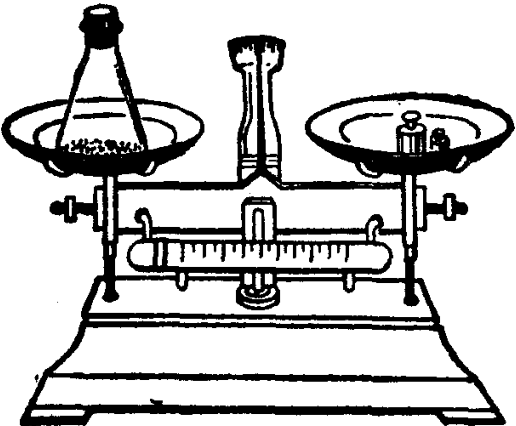
\includegraphics[width=6cm]{../pic/czhx1-ch1-13}
        \caption{\begin{minipage}[t]{3cm} % 原本这里可以不用 minipage,但为了和 1-14 对齐,也采用 minipage。
            白磷燃烧前后\\
            质量的测定
        \end{minipage}}\label{fig:1-13}
    \end{minipage}
    \qquad
    \begin{minipage}[b]{7cm}
        \centering
        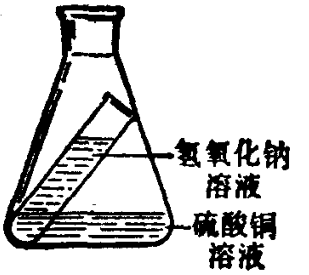
\includegraphics[width=4cm]{../pic/czhx1-ch1-14}
        \caption{\begin{minipage}[t]{5cm}
            氢氧化钠溶液跟硫酸铜\\
            溶液反应的装置
        \end{minipage}}\label{fig:1-14}
    \end{minipage}
\end{figure}


\begin{shiyan}
    把盛有无色氢氧化钠溶液的短试管,小心地放入盛有蓝色硫酸铜溶液的锥形瓶里(图 \ref{fig:1-14}) ,
    再把放有短试管的锥形瓶放在天平的一个托盘上,用砝码平衡。
    然后拿起锥形瓶并使它倾斜,使氢氧化钠溶液倒入硫酸铜溶液里,
    两种溶液接触,立即发生化学反应,生成蓝色沉淀物。
    再把锥形瓶放回托盘上,观察天平两边是否平衡。
\end{shiyan}

从上面两个实验都可以看出,天平两边都仍然是平衡的,说明反应前后物质的质量总和没有变化。
无数的实验证明,\zhongdian{参加化学反应的各物质的质量总和,
等于反应后生成的各物质的质量总和。这个规律叫做质量守恒定律。}

为什么物质在发生化学反应前后,各物质的质量总和相等呢?
这是因为化学反应的过程,就是参加反应的各物质(反应物)的原子,重新组合而生成其它物质(生成物)的过程。
也就是说,在一切化学反应里,反应前后原子的种类没有改变,原子的数目也没有增减,
所以,化学反应前后各物质的质量总和必然相等。


\subsection{化学方程式}

在工农业生产和科学实验里,通常都用分子式来表示有关的化学反应。
如木炭在氧气里燃烧,生成二氧化碳,这个反应可表示如下:
\begin{fangchengshi}
    \ce{ C + O2 = CO2 }
\end{fangchengshi}

这种\zhongdian{用分子式来表示化学反应的式子,叫做化学方程式。}

书写化学方程式要注意两个原则:
一是必须以客观事实作为基础,决不能凭空设想,
随便臆造事实上不存在的化学反应或不存在的物质,也不能任意编造分子式;
二是要遵循质量守恒定律,等号两边各种原子的总数必须相等。

下面以磷在空气里燃烧生成五氧化二磷的反应为例,说明书写化学方程式的步骤。

1. 写出反应物和生成物的分子式:
根据实验的事实,在式子的左边写出反应物的分子式,在式子的右边写出生成物的分子式,
如果反应物或生成物不止一种,就分别用加号把它们连接起来,并在式子左、右两边之间划一条短线。
\begin{fangchengshi}
    \ce{ P + O2 - P2O5 }
\end{fangchengshi}

2. 配平化学方程式:
写化学方程式必须遵循质量守恒定律。
因此,式子左、右两边的分子式前面要配上适当的系数,使式子左、右两边的每一种元素的原子总数相等。
化学上把这个过程叫做化学方程式的配平。
配平化学方程式的方法有很多种,上面的式子一般可用求最小公倍数法来确定系数。
在这个式子里,左边的氧原子数是 $2$, 右边的氧原子数是 $5$, 两数的最小公倍数是 $10$,
因此,在 \ce{O2} 前面要配上系数 $5$, 在 \ce{P2O5} 前面配上系数 $2$。
\begin{fangchengshi}
    \ce{ P + 5O2 - 2P2O5 }
\end{fangchengshi}

式子右边的磷原子数是 $4$, 左边的磷原子数是 $1$,因此,应在 $\ce{P}$ 的前面配上系数 $4$。
\begin{fangchengshi}
    \ce{ 4P + 5O2 - 2P2O5 }
\end{fangchengshi}

式子两边各元素的原子数配平后,把短线改成等号。
\begin{fangchengshi}
    \ce{ 4P + 5O2 = 2P2O5 }
\end{fangchengshi}

如果在特定条件下进行的反应,还必须把外界条件,如点燃、加热(用 “$\Delta$” 号表示)、
催化剂等等,写在等号的上方\footnote{如有两种以上的条件, 一般把加热(即$\Delta$)写在等号的下方。}。
如果生成物中有沉淀或者气体产生,般应该用 “\ce{v}” 号或者 “\ce{^}” 号表示出来。
例如:
\begin{fangchengshi}
    \ce{ 4P + 5O2 \xlongequal{\text{点燃}} 2P2O5 } \\
    \ce{ $\underset{\text{氯酸钾}}{\ce{2KClO3}}$
         $\xlongequal[\Delta]{\ce{MnO2}}$
         $\underset{\text{氯化钾}}{\ce{2KCl}}$
         + 3O2 ^
    } \\
    \ce{ $\underset{\text{硫酸铜}}{\ce{CuSO4}}$
         +
         $\underset{\text{氢氧化钠}}{\ce{2NaOH}}$
         =
         $\underset{\text{硫酸钠}}{\ce{Na2SO4}}$
         +
         $\underset{\text{氢氧化铜}}{\ce{Cu(OH)2}}$ v
    }
\end{fangchengshi}

化学方程式表示什么物质参加反应,结果生成什么物质,
还可以表示反应物、生成物各物质之间的质量比。
例如:
\begin{center}
    \begin{tblr}{columns={mode=math, c},
        rowsep=0pt,
    }
        \ce{4P} & + & \ce{5O2} & = & \ce{2P2O5}  \\
        4 \times 31 & : & 5 \times 16 \times 2 & : & 2(31 \times 2 + 16 \times 5) \\
        124 & : & 160 & : & 284
    \end{tblr}
\end{center}

就是说,每 $124$ 份质量的磷跟 $160$ 份质量的氧化合,能够生成 $284$ 份质量的五氧化二磷。


在工农业生产和科学实验上,广泛应用化学方程式来进行计算。



\begin{xiti}

\xiaoti{用质量守恒定律解释下面两种现象:}
\begin{xiaoxiaotis}

    \xxt{镁带在空气里燃烧后,生成物的质量比镁带的质量增加了;}

    \xxt{煤燃烧后留下的煤灰的质量,比煤的质量减少了。}

\end{xiaoxiaotis}

\xiaoti{写出下列反应的化学方程式:}
\begin{xiaoxiaotis}

    \xxt{镁在氧气里燃烧生成氧化镁。}

    \xxt{碳酸氢铵(\ce{NH4HCO3}) 分解生成氨气(\ce{NH3})、二氧化碳和水。}

    \xxt{硫在氧气里燃烧生成二氧化硫(\ce{SO2})。}

    \xxt{氧气跟乙炔(\ce{C2H2})起反应发生燃烧,生成二氧化碳和水。}

    \xxt{氢气跟氮气在一定条件(高温、高压、催化剂)下反应生成氨气(\ce{NH3})。}

\end{xiaoxiaotis}


\xiaoti{配平下列反应的化学方程式,并指出它们各属于哪种反应类型。}
\begin{xiaoxiaotis}

    \xxt{\ce{H2O - H2 + O}}

    \xxt{\ce{C + CO2 - CO}}

    \xxt{\ce{Fe + O2 - Fe3O4}}

    \xxt{\ce{KMnO4 - K2MnO4 + MnO2 + O2}}

\end{xiaoxiaotis}


\xiaoti{写出氧化汞分解的化学方程式,并指出反应物和生成物各物质之间的质量比。}

\end{xiti}


